% TODO: reorganizar este apêndice para fazer mais sentido

\begin{apendicesenv}
\partapendices

\chapter{Descrição matemática do modelo de micelas gigantes}

\section{Introdução e motivação}

% TODO: colocar as referências.
Esta seção mostrará as equações utilizadas para descrever o modelo de espalhamento de micelas gigantes. As equação foram baseadas numa série de artigos de X, Y, Z. Aqui, esses artigos serão agrupados, de modo a facilitar o entendimento do modelo.

Porém, essa descrição matemática é de menor aplicabilidade, pois é necessário transcrever as equações em código que consiga realizar ajustes. Essa tarefa não é trivial, especialmente para não especialistas. Logo, será disponibilizado, na seção X, uma transcrição dessas equações, na linguagem Python.

% TODO: colocar a seção onde o modelo foi utilizado
% TODO: colocar a seção onde a descrição de Python foi escrita
% TODO: reescrever essas equações, colocando os termos qe são texto em \text e o resto normal

\section{Resumo do modelo}

O modelo descreve cadeias alongadas caroço-casca (\emph{core-shell}) de Kratky-Porod, considerando volume excluído, com interações intercadeias modeladas pelo modelo PRISM (\emph{Polymer Reference Interaction Site Model}). No total, a equação de intensidade de espalhamento $I$ em função do vetor de espalhamento \q ($I(q)$, Eq. \ref{eqn:AP_saxs_MG_superficial}) possui 13 parâmetros, descritos na tabela \ref{tab_ap:simbolos}.

\begin{equation}
I = f(q, scale, d_{head}, r_{core}, \rho_{rel}, \sigma, back, L, k_L, \varepsilon, D_{CQ}, \nu_{RPA}, SC_{pow}, exp_{pow})
\label{eqn:AP_saxs_MG_superficial}
\end{equation}
% TODO: colocar refs às equações que definem alguns desses termos
\begin{table}
    \IBGEtab%
    {\caption{Símbolos e parâmetros utilizados no modelo, e seus significados}
     \label{tab_ap:simbolos} }%
    {\begin{tabular}{r p{8cm}}
    	\toprule
     Símbolo 			& Descrição        						\\
     \midrule
     $I$					& Intensidade de RX espalhado			\\
     \q					& Vetor de espalhamento					\\
     \midrule
     $scale$				& Fator de escala						\\
     $d_{head}$			& Espessura do \emph{shell}				\\
     $r_{core}$			& Raio do \emph{core}					\\
     $\rho_{rel}$		& Diferença de densidade eletrônica entre \emph{core} e \emph{shell} \\
     $\sigma$			& Fator de \emph{smearing}, o quão definido é o limite entre regiões \\
     $back$				& Constante referente ao \emph{background} \\
     $L$					& Comprimento de contorno das cadeias 	\\
     $k_L$				& Comprimento de \emph{Kuhn} das cadeias, igual ao dobro do comprimento de correlação \\ % TODO: Achar o que é esse comprimento exatamente
     $\varepsilon$			& Excentricidade radial das micelas		\\
     $D_{CQ}$			& Distância de correlação das micelas 	\\
     $\nu_{RPA}$			& Fator de concentração					\\
     \midrule
     $SC_{pow}$			& Fator de escala (pre-exponencial) da exponencial em baixo q\\
     $exp_{pow}$			& Fator exponencial, relativo à inclinação na escala log\\
     \bottomrule
    \end{tabular}}%
    {}%
\end{table}

A equação geral do modelo, e a descrição de seus fatores, estão descritos na Eq.\ref{eqn:AP_saxs_MG_geral} e na Tab. \ref{tab_ap:fatores_geral}.

\begin{equation}
I = \frac{scale\left(F_{KPchain_{ExV}}F_{rod_{CS}}\right)}{1 + \nu_{RPA} F_{sphere}\left( D_{CQ}\right) F_{KPchain_{ExV}}} + back + scale_{pow}^{-exp_{pow}}
\label{eqn:AP_saxs_MG_geral}
\end{equation}

\begin{table}
    \IBGEtab%
    {\caption{Parâmetros da equação \ref{eqn:AP_saxs_MG_geral}}
     \label{tab_ap:fatores_geral} }%
    {\begin{tabular}{r p{8cm}}
    \toprule
    Termo 			& Descrição        						\\
    \midrule
    $F_{KPchain_{ExV}}$  & Fator forma de cadeias de Kratky-Porod com volume excluído \\
    $F_{rod_{CS}}$		 & Fator forma da seção transversão de um bastão	\\
    $F_{sphere}(D_{CQ})$ & Fator forma de uma esfera, cujo raio é a distância de correlação \\
    \bottomrule%
    \end{tabular}}
    {}%
\end{table}


Já o modelo do PRISM é descrito pela Eq. \ref{eqn:AP_saxs_PRISM}. Note a similaridade com a Eq \ref{eqn:AP_saxs_MG_geral}.

\begin{equation}
I_{PRISM}= \frac{\varphi V_{mic}F_{wc}(q)F_{cs}(q)}{1 + \nu F_{rod}(qL_{c(q)})F_{wc}(q)}
\label{eqn:AP_saxs_PRISM}
\end{equation}

\begin{table}
    \IBGEtab{%
      	\caption{Termos da equação \ref{eqn:AP_saxs_PRISM}}
    \label{tab_ap:PRISM_geral}}%
    {%
     \begin{tabular}{r p{8cm}}
     \toprule
     Termo 			& Descrição        						\\
     \midrule
     $\varphi$		& Fração volumétrica \\ % TODO: checar
     $V_{mic}$		& Volume da micela   \\
     $F_{wc}$		& Fator forma de uma \emph{wormlike chain} \\
     $F_{cs}$		& Fator forma de uma seção transversal de cilindro \\ % TODO: checar se é cilindro
     $F_{rod}$		& Fator forma de um bastão infinitamente longo \\
     $L_{c(q)}$		& $=6\xi$, comprimento característico \\
     $\xi$			& Comprimento de correlação da função $c(q) \approx F_{rod}$ \\
     \bottomrule
     \end{tabular}}%
     {}%
\end{table}


A partir disso, podemos começar a adentrar nos termos.

\section{Descrição detalhada do modelo}

O modelo será dividido em duas partes, uma referente à cadeia micelar, $F_{wc}$ e outra referente à seção transversal da cadeia, $F_{cs}$.

\subsection{Fator forma das cadeias \emph{wormlike}, $F_{wc}$}
\label{sec:equacoes_Fwc}

\begin{equation}
F_{wc} = \left[\left(1 - \chi\right)F_{chain_{ExV}} + \chi F_{rod}\right]\Gamma
\label{eqn:AP_Fwc}
\end{equation}

% TODO: colocar a equação do \Gamma
A equação \ref{eqn:AP_Fwc} pode ser simplificada dependendo da faixa de \q. A região de \q intermediária precisa ser descrita pelo termo $\chi$ (Eq. \ref{eqn:AP_chi}) e corrigida por $\Gamma$. Esses parâmetros são obtidos por simulações de Monte Carlo.

\begin{equation}
	F_{\text{wc}} \approx 
		\begin{cases}
			F_{\text{chain}_{\text{ExV}}}		& \text{q baixo}  \\
			F_{\text{rod}}						& \text{q alto}
		\end{cases}
\end{equation}

%	\begin{longtable}[c]{r p{12cm}}
%		\toprule
%		Termo 			& Descrição        						\\
%		\midrule
%		$\chi$			& Região de \emph{crossover} \\
%		$\Gamma$		& Correção da região de crossover. \\
%		\bottomrule
%		\caption{Termos da equação \ref{eqn:AP_Fwc}}
%		\label{tab_ap:Fwc} 
%	\end{longtable}

\subsubsection{Fator de correção $\chi$}
O termo $\chi$ é descrito pela equação \ref{eqn:AP_chi}, que por sua vez é dependente da equação \ref{eqn:AP_xi}.

\begin{equation}
\chi = \exp{\xi^{-5}}
\label{eqn:AP_chi}
\end{equation}

% todo: achar o significado do termo b
\begin{equation}
\xi = q k_L\left(\frac{\pi b}{1,103L}\right)^{3/2}\left(\frac{\left<R_g^2\right>}{k_L^2}\right)^{1,282}
\label{eqn:AP_xi}
\end{equation}

\noindent onde $\left<R_g^2\right>$ é a média do \emph{ensemble} do quadrado do raio de giro das cadeias, no modelo.

\subsubsection{Fator forma de cadeias com volume excluído, $F_{chain_{ExV}}$}
\label{sec:F_chain_ExV_equacoes}
O termo $F_{chain_{ExV}}$ possui a seguinte forma (Eq. \ref{eqn:AP_FchainExV})

% TODO: verificar se o \nu aqui é o \nu_RPA
\begin{multline}
F_{chain_{ExV}} = w(qR_g)F_{Debye}(q,L,k_L) + \left[1 - w(q R_g)\right] \\ \left[C_1(q R_g)^{\frac{1}{\nu}} + C_2(q R_g)^{-\frac{2}{\nu}} + 
C_3(q R_g)^{-\frac{3}{\nu}}\right]
\label{eqn:AP_FchainExV}
\end{multline}
% todo: colocar o valor de \nu, que está na Eq. S_EXV_APP
% todo: incluir aqui uma tabela com os termos e as equações

O termo $F_{Debye}$, por sua vez, é dado pela Eq. \ref{eqn:AP_fdebye}.
\begin{equation}
F_{Debye} = 2 \left(\frac{e^{-u} + u - 1}{u^2}\right)
\label{eqn:AP_fdebye}
\end{equation}

\noindent onde $u = R_g^2q^2$. $R_g$ é a raiz quadrada do raio de giro médio ao quadrado, $R_g = \left<R_g^2\right>^{1/2}$, considerando o volume excluído. Por sua vez, esse valor é dado pela Eq. \ref{eqn:AP_Rg2}

% Achar o que significam os termos faltantes aqui.
\begin{equation}
\left<R_g^2\right> = \alpha \left(\frac{L}{k_L}\right)^2\left<R_g^2\right>_0
\label{eqn:AP_Rg2}
\end{equation}

O termo $w$ é uma equação empírica, da forma: (Eq \ref{eqn:AP_w})

\begin{equation}
w(x) = \frac{\left[1 + \frac{\tanh(x-C_4)}{C_5}\right]}{2}
\label{eqn:AP_w}
\end{equation}

As constantes $C_1$, $C_2$, $C_3$, $C_4$ e $C_5$ foram obtidas a partir de um ajuste, e estão na tabela \ref{tab_ap:C1C5}, assim como o valor de $\nu$.
\begin{table}
    \IBGEtab%
    {\caption{Constantes}
    \label{tab_ap:C1C5} }%
    {\begin{tabular}{r p{2cm}}
      \toprule
      Constante 	& Valor \\
      \midrule
      $C_1$			&  1,220	\\
      $C_2$			&  0,4288	\\
      $C_3$			&  -1,651	\\
      $C_4$			&  1,523	\\
      $C_5$			&  0,1477 	\\	
      $\nu$			&  0,585	\\					
      \bottomrule
    \end{tabular}}% todo: encontrar de onde vem o \nu
    {}%
\end{table}


\subsubsection{Fator de correção $\Gamma$}

O fator de correção $\Gamma$ (Eq. \ref{eqn:AP_Gamma}) é dependente de dois conjuntos de constantes, $A$ (Eq. \ref{eqn:AP_Ai}) e B (Eq. \ref{eqn:AP_Bi}) determinadas empiricamente (Tab \ref{tab_ap:AiBi}).

\begin{equation}
\Gamma\left( q,L,k_{L} \right) = 1 + \left( 1 - \chi \right)\sum_{i = 2}^{5}{A_{i}\xi^{i}} + \chi\sum_{i = 0}^{2}{B_{i}\xi^{- i}}
\label{eqn:AP_Gamma}
\end{equation}

\begin{equation}
A_{i} = \sum_{j = 0}^{2}{a_{1}\left( i,j \right)\left( \frac{L}{k_{L}} \right)^{- j}\exp\left( - \frac{10k_{L}}{L} \right)} + \sum_{j = 1}^{2}{a_{2}\left( i,j \right)\left( \frac{L}{k_{L}} \right)^{j}\exp\left( - \frac{2L}{k_{L}} \right)}
\label{eqn:AP_Ai}
\end{equation}

\begin{equation}
B_{i} = \sum_{j = 0}^{2}{b_{1}\left( i,j \right)\left( \frac{L}{k_{L}} \right)^{- j}\ } + \sum_{j = 1}^{2}{b_{2}\left( i,j \right)\left( \frac{L}{k_{L}} \right)^{j}\exp\left( - \frac{2L}{k_{L}} \right)}
\label{eqn:AP_Bi}
\end{equation}

\begin{table}[h]
    \IBGEtab%
    {\caption{Constantes utilizadas para o cálculo de $\Gamma$}
    \label{tab_ap:AiBi}}%
    {\begin{tabular}{r l | r l | r l | r l}
    \toprule
    $a_1$(2,0) & --0.1222 & $a_2$(2,1) & 0.1212 & $b_1$(0,0) &
    --0.0699 & $b_2$(0,1) & --0.5171\\
    $a_1$(3,0) & 0.3051 & $a_2$(3,1) & --0.4169 & $b_1$(1,0) & --0.09
    & $b_2$(1,1) & --0.2028\\
    $a_1$(4,0) & --0.0711 & $a_2$(4,1) & 0.1988 & $b_1$(2,0) &
    0.2677 & $b_2$(2,1) & --0.3112\\
    $a_1$(5,0) & 0.0584 & $a_2$(5,1) & 0.3435 & $b_1$(0,1) & 0.1342
    & $b_2$(0,2) & 0.6950\\
    $a_1$(2,1) & 1.761 & $a_2$(2,2) & 0.0170 & $b_1$(1,1) & 0.0138 &
    $b_2$(1,2) & --0.3238\\
    $a_1$(3,1) & 2.252 & $a_2$(3,2) & --0.4731 & $b_1$(2,1) & 0.1898
    & $b_2$(2,2) & --0.5403\\
    $a_1$(4,1) & --1.291 & $a_2$(4,2) & 0.1869 & $b_1$(0,2) & --0.2020
    & &\\
    $a_1$(5,1) & 0.6994 & $a_2$(5,2) & 0.3350 & $b_1$(1,2) & --0.0114
    & &\\
    $a_1$(2,2) & --26.04 & & & $b_1$(2,2) & 0.0123 & &\\
    $a_1$(3,2) & 20.00 & & & & & &\\
    $a_1$(4,2) & 4.382 & & & & & &\\
    $a_1$(5,2) & 1.594 & & & & & &\\
    \bottomrule
   \end{tabular} }%
    {}%
\end{table}

\subsubsection{Fator forma de um cilindro $F_{rod}$}

O fator forma de um cilindro segue a equação \ref{eqn:AP_Frod}.

\begin{equation}
F_{rod}(q, L) = \frac{2Si(qL)}{qL} - \frac{4\sin^2\frac{qL}{2}}{q^2L^2}
\label{eqn:AP_Frod}
\end{equation}

\noindent onde $Si$ é a função-integral de seno (Eq. \ref{eqn:AP_Si})

\begin{equation}
Si(x) = \int_0^x \frac{\sin t}{t}dt
\label{eqn:AP_Si}
\end{equation}

% TODO: verificar se F_CS é de fator da seção de um cilindro. CS é cross section mesmo.
\subsection{Fator forma da seção transversal de um cilindro $F_{cs}$}

O fator forma da seção transversal de um cilindro é descrito pela equação \ref{eqn:AP_Fcs}. Seus parâmetros se encontram na tabela \ref{tab_ap:Fcs}

\begin{equation}
F_{\text{cs}} = \frac{2}{\pi}\int_{0}^{\frac{\pi}{2}}%
%
\left[ \left(\rho_{S} - \rho_{w} \right) \frac{2J_1 \left( qR_{s}\left( \varepsilon,\theta \right) \right)}{qR_{s}\left( \varepsilon,\theta \right)} % 
%
+  %
%
\frac{\pi\varepsilon R_c^2}{\pi\varepsilon R_s^2}\left( \rho_c - \rho_s \right)	%
%
\frac{2J_1\left( qR_{c}\left( \varepsilon,\theta \right) \right)}{qR_{c}\left( \varepsilon,\theta \right)}\  \right]^2 d\theta
\label{eqn:AP_Fcs}
\end{equation}

% Todo: padronizar essas equações
% Todo: verificar se o \varepsilon é a excentricidade
% Todo: verificar se Rc e Rs são funções de \varepsilon e \theta

\begin{table}
    \IBGEtab{\caption{Parâmetros para a equação \ref{eqn:AP_Fcs}}
    \label{tab_ap:Fcs} }%
    {\begin{tabular}{r l}
            \toprule
            Parâmetro 			& Significado \\
            \midrule
            $\rho_S$			&  Densidade eletrônica do \emph{shell} \\
            $\rho_C$			&  Densidade eletrônica do \emph{core}  \\
            $\rho_w$			&  Densidade eletrônica da água			\\
            $R_S$			& Raio do \emph{shell} 						\\
            $R_C$			& Raio do \emph{core}						\\
            $J_1$			&  Função de Bessel do primeiro tipo e de primeira ordem\\
            $C_4$			&  1,523	\\
            $C_5$			&  0,1477 	\\						
            \bottomrule
        \end{tabular}}%
    {}%
\end{table}

Os termos $R_S$ e $R_C$ podem ser calculados pelas expressões \ref{eqn:AP_Rs} e \ref{eqn:AP_Rc}

\begin{equation}
R_C(\varepsilon\theta) = \sqrt{R_C^2\sin^2\theta + \varepsilon^2R_c^2\cos^2\theta}
\label{eqn:AP_Rc}
\end{equation}

\begin{equation}
R_C = \sqrt{\frac{V_{\text{surf, apolar}}}{V_{\text{surf, total}}}}R_S
\label{eqn:AP_Rs}
\end{equation}

\noindent onde V é o volume molecular das regiões do surfactante.


\chapter{Códigos}

	Neste apêndice serão descritos alguns dos métodos computacionais criados durante a execução deste doutorado. Todos os scripts foram escritos na linguagem Python. O aluno fortemente recomenda essa linguagem para outros que desejam tratar, visualizar e entender seus dados. Python possui uma sintaxe simples, mas poderosa, grande número de pacotes matemáticos e científicos de qualidade, e é totalmente gratuito. Em especial, a conjunção de \emph{Jupyter Notebooks} (extensão \texttt{ipynb}) com um \emph{kernel} de Python é uma ferramenta muito poderosa e conveniente.
	
	Um curso de Python com foco em tratamento de dados foi elaborado pelo aluno, e se encontra disponível em um repositório no Github\footnote{\href{https://github.com/KarlClinckspoor/CursoPython}{https://github.com/KarlClinckspoor/CursoPython}}. Em brevo, o curso possui a seguinte estrutura:
	
	\begin{enumerate}
		\item ``Hello world'', strings, obtendo ajuda
		\item Operações matemáticas, variáveis
		\item Estruturas de dados
		\item Condicionais e loops
		\item Instalando e carregando módulos
		\item Definindo funções
		\item Matemática computacional com \emph{numpy}
		\item Carregando e manipulando dados com \emph{pandas}
		\item Criando gráficos com \emph{pyplot}
		\item Tópicos avançados de tratamento de dados
		\item Tópicos adicionais
	\end{enumerate}

\section{Descrição do modelo de micelas gigantes em Python}

	Esta seção mostrará as equações do modelo de micelas gigantes, utilizado neste trabalho. O modelo foi criado pelo Prof. Jan Skov Pedersen, em Fortran 77, e disponibilizado para o aluno para realizar os ajustes das curvas obtidas no ESRF. O aluno então transcreveu o código de Fortran para Python, uma linguagem mais clara, e criou um pequeno programa interativo que relaciona o modelo com seus parâmetros. O programa consegue também comparar uma curva teórica com dados experimentais, de modo a fornecer um bom chute inicial para o ajuste das curvas.
	
\begin{figure}[H]
	\centering
	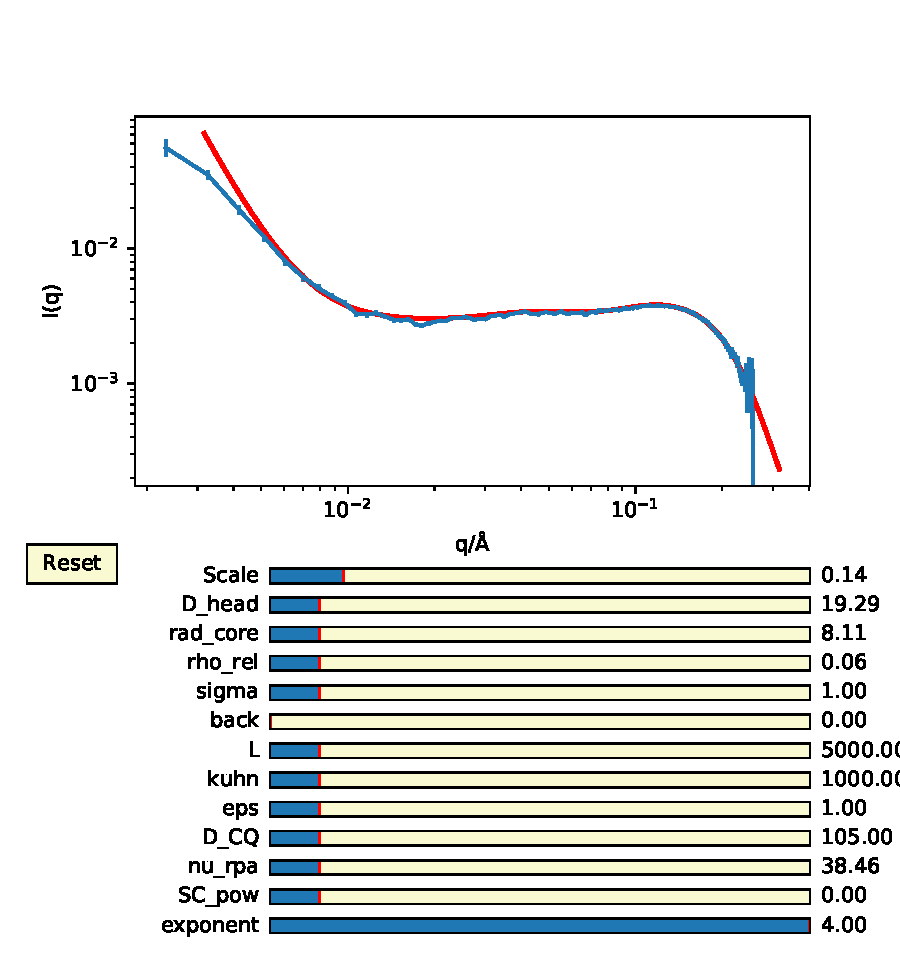
\includegraphics[width=0.7\textwidth]{imagens/saxs/Modelo_dado_SAXS_python}
	\caption{Dado real (azul) e modelo (vermelho) junto com os parâmetros de ajuste utilizados no modelo}
	\label{fig:saxs_modelo_dado_saxs_python}
\end{figure}

	% todo: colocar uma imagem do modelo em ação
	
	Uma das motivações para realizar essa tarefa foi a grande dificuldade de nosso grupo utilizar SAXS para estudar micelas. Não há especialistas na região que conhecem modelagem de micelas gigantes. Além disso, escrever um modelo computacional baseando-se somente as equações matemáticas é uma tarefa muito difícil. O modelo computacional, apesar de menos compacto em sua notação, é mais fácil de ser utilizado pois os passos são bastante detalhados, o que também facilita o entendimento de novos alunos.
	
	\subsection{Fator $F_{KPchain_{ExV}}$}
	As equações da seção \ref{sec:equacoes_Fwc} relevantes ao cálculo do fator de cadeias com volume excluído então descritas nos códigos a seguir (listas \ref{lst:cadeia_KP_1}, \ref{lst:cadeia_KP_2}, \ref{lst:cadeia_KP_3}, \ref{lst:cadeia_KP_Debye}, \ref{lst:cadeia_KP_SI}).
	
	\begin{listing}[H]
		\inputminted{python}{./python/cadeia_kratky_porod_inicial_1.py}
		\caption{Cálculo do fator de cadeias de Kratky-Porod com volume excluído (Parte 1/3)}
		\label{lst:cadeia_KP_1}
	\end{listing}

	\begin{listing}[H]
		\inputminted{python}{./python/cadeia_kratky_porod_inicial_2.py}
		\caption{Cálculo do fator de cadeias de Kratky-Porod com volume excluído (Parte 2/3)}
		\label{lst:cadeia_KP_2}
	\end{listing}

	\begin{listing}[H]
		\inputminted{python}{./python/cadeia_kratky_porod_inicial_3.py}
		\caption{Cálculo do fator de cadeias de Kratky-Porod com volume excluído (Parte 3/3)}
		\label{lst:cadeia_KP_3}
	\end{listing}

	\begin{listing}[H]
		\inputminted{python}{./python/cadeia_kratky_porod_inicial_4.py}
		\caption{Cálculo do fator de Debye}
		\label{lst:cadeia_KP_Debye}
	\end{listing}

	\begin{listing}[H]
		\inputminted{python}{./python/cadeia_kratky_porod_inicial_5.py}
		\caption{Cálculo numérico da integral cardinal}  % todo: encontrar um nome melhor
		\label{lst:cadeia_KP_SI}
	\end{listing}

	
\section{Descrição e uso do software de tratamento de curvas de fluxo}

Para o tratamento de curvas de fluxo de fluidos pseudoplástico, foi desenvolvido um software que realiza o ajuste das curvas por um modelo simplificado e três modelos mais complexos, de forma a contornar erros experimentais. Esse software acelera em várias vezes a velocidade de tratamento. Nesta seção, será descrito o algoritmo que o programa faz para os ajustes, e será dada uma breve introdução para o uso do software tanto num ambiente Python, como um script \emph{standalone}.

\section{Softwares miscelâneos para tratamento de dados}
\end{apendicesenv}

%\begin{anexosenv}
%
%% Imprime uma página indicando o início dos anexos
%\partanexos
%
%% ---
%\chapter{Morbi ultrices rutrum lorem.}
%% ---
%\lipsum[30]
%
%% ---
%\chapter{Cras non urna sed feugiat cum sociis natoque penatibus et magnis dis
%parturient montes nascetur ridiculus mus}
%% ---
%
%\lipsum[31]
%
%% ---
%\chapter{Fusce facilisis lacinia dui}
%% ---
%
%\lipsum[32]
%
%\end{anexosenv}
